\subsection{The Pixel-By-Pixel Tagging Algorithm}

This algorithm is a modified version of the image labelling algorithm presented in \cite{imglabelseq}. The input is the image captured by the image sensor, and the output is an array containing the centroids of 4-connected regions of bright pixels in the input image in the frame centered at the center of the image and scaled to the size of the pixels (rather than in units of pixel lengths), along with Star IDs that are set as an integer between 1 and N, with N being the number of stars detected by the algorithm. These are allotted in the order of the position of the stars in the output array.

We now describe the algorithm:
\begin{enumerate}
    \item A row of zeros is added to the north of the input image and a column of zeros is added to both the left and right of the input image. The algorithm iterates over the input image from the top left to the bottom right of the image (excluding the added zero elements)
    \item Whenever the algorithm encounters a bright pixel, it checks the pixel to the north and to the left. We store $ \sum C_{i_{x}}Intensity_{i}, \sum C_{i_{y}}Intensity_{i}, \sum Intensity_{i} $, the number of pixels and the flag for each tag\footnote{Note that a bright pixel that has already been inspected by the algorithm will \emph{always} have a tag.}.
    
    The following cases are encountered while checking the neighbouring pixels:
    \begin{enumerate}
        \item If both of them are bright, it checks their tags
        \begin{enumerate}
            \item If both of the tags are the same, the data of the pixel is added to the data of the corresponding tag
            \item If both of them are different, it sets flags to note the equivalence relationship, since they get connected at a pixel. We also have a table to list the tags associated with every flag. It checks the flags associated with both flags.
            \begin{itemize}
                \item If both the tags have the same flag, nothing needs to be done
                \item If only one of the tags has a flag, it flags the other tag with that flag. The newly flagged tag is added to the table in the corresponding row
                \item If both the tags have different flags, it merges the two rows in the table to the one with the smaller flag and updates the flag of all tags in the row
                \item If none of them have flags, it creates a new flag and flag the tags, and adds them to the new row in the table
            \end{itemize}
        Regardless of what the flags are, it adds the data of the pixel to the data of the tag of the pixel to the north and tags it with the same.
        \end{enumerate}
        \item If only one of them is bright, the pixel is tagged with the corresponding tag and the data is added to the data of that tag
        \item If none of them are bright, it checks the pixel to the right and the one to the right of the one to the north\footnote{This is done to reduce the unnecessary creation of new tags and the resulting conflicts between tags that will eventually get connected at some pixel. The testing done so far has suggested that this is fairly effective in cutting down on the use of flags and the resulting merge.}.
            \begin{itemize}
                \item If both of those are bright, the pixel is tagged with the tag of the pixel to the right of the one to the north. 
                \item If not, the pixel is assigned a new tag and the data is added to the corresponding tag's data
            \end{itemize}
    \end{enumerate}
    \item After each pixel is tagged, it no longer needs the input image, all the data we need is stored with the data of each tag. It goes through the flags for each tag and combines the data of the flagged ones. 
    \item It then goes through all the data corresponding to the merged tags and the unflagged tags and filters out the ones that have too few or too many pixels and finds the centroids for the remaining regions.
    \item The Star IDs are then added to the array and this, along with the number of regions, is given as the final output.
\end{enumerate}
The flowchart for this algorithm is shown in Figure \ref{FC:pbp_centroiding}
\newpage
\begin{Flowchart}
    \centering
    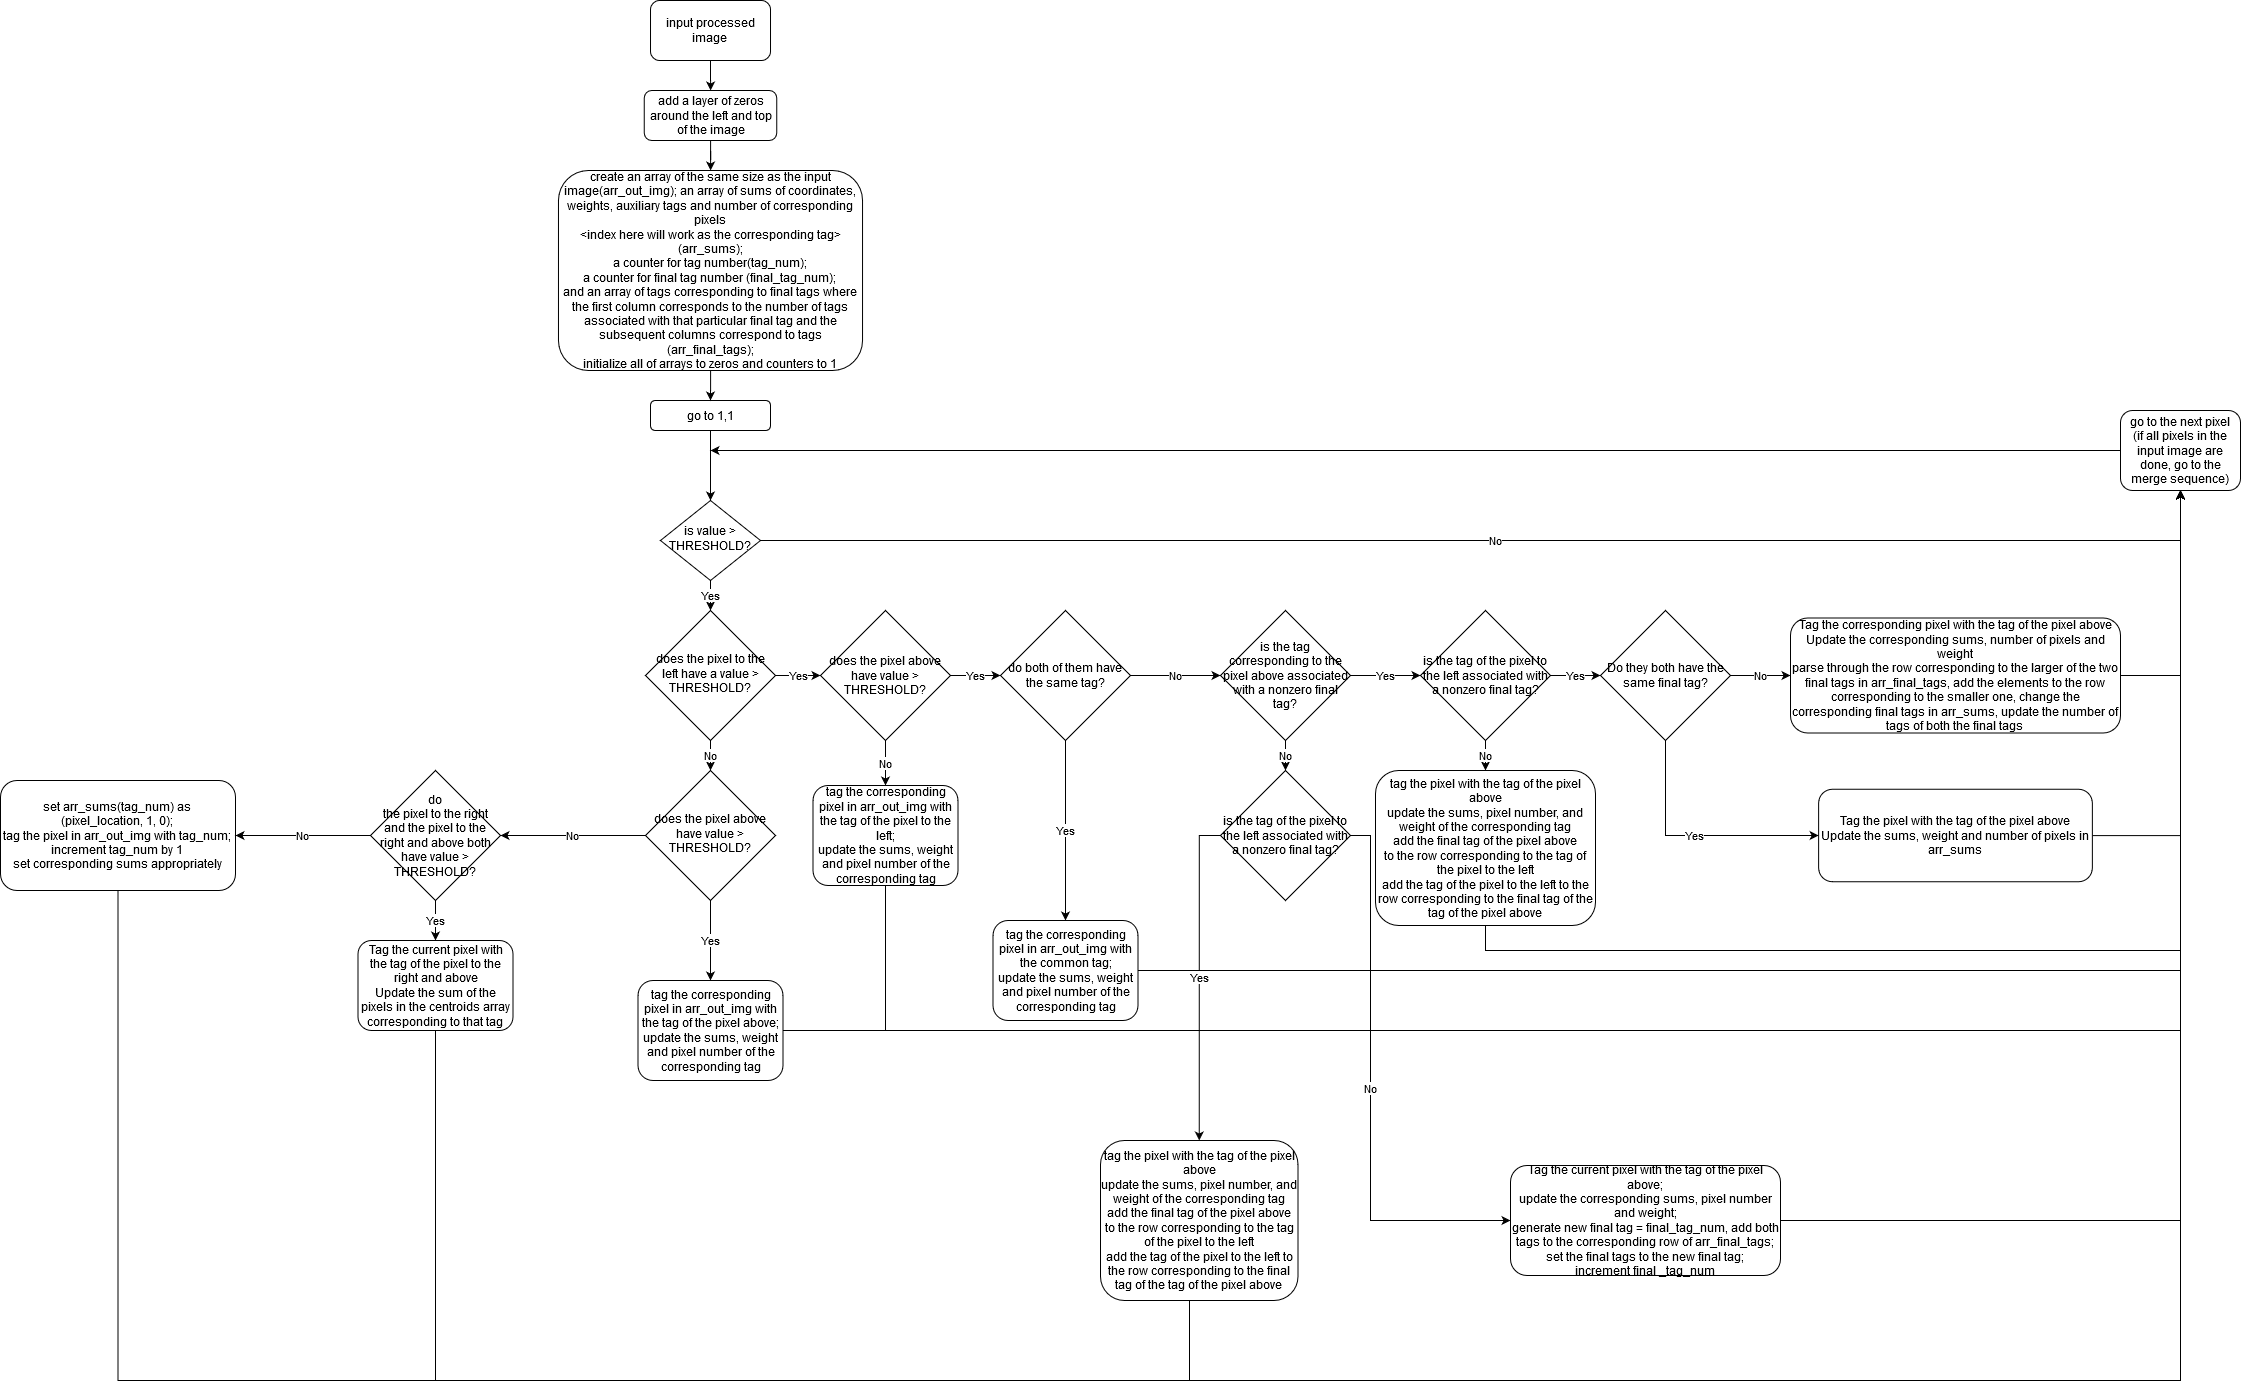
\includegraphics[width=\textwidth]{Figures/Electrical/centroiding_2.png}
    \caption{Pixel-by-Pixel Tagging Algorithm}
    \label{FC:pbp_centroiding}
\end{Flowchart}